%\begin{figure}
%\resizebox{\textwidth}{!}{
%\begin{tikzpicture}
%
%
%\draw  [fill=blue,fill opacity=0.2](7.6,-1.45) rectangle (14.65,3.5);
%\draw   [fill=blue,fill opacity=0.2](1.55,-1.45) rectangle (6.2,3.5);
%\draw   [fill=blue,fill opacity=0.2](-2.9,-1.45) rectangle (0.15,3.5);
%
%\draw  [fill=white](-2.3,0) rectangle (-0.8,1)node[pos=.5]{\large Human};
%\draw  [fill=white](-2.3,2.05) rectangle (-0.8,3.05)node[pos=.4, above,xshift=5]{\large Haptic};
%\draw  (-2.3,2.05) rectangle (-0.8,3.05)node[pos=.5, below,xshift=0]{\large Device};
%\draw  [fill=white](2.2,2.05) rectangle (3.25,3.05)node[pos=.5]{\large K};
%\draw  [fill=white](2.25,0) rectangle (5.3,1)node[pos=.5,above]{Coordinate}node[pos=.5,below]{Transform};
%
%\draw  (0.3,0) rectangle (1.4,1)node[pos=.5]{ Delay};
%\draw  (0.3,2.05) rectangle (1.4,3.05)node[pos=.5]{ Delay};
%\draw  (6.35,2.05) rectangle (7.4,3.05)node[pos=.5]{ Delay};
%
%\draw [->,line width=1pt] (-1.55,2.05) -- (-1.55,1) node [pos=0.5,left] {F};
%\draw [->,line width=1pt] (-0.8,0.5) -- (0.3,0.5) node [pos=0.5,above] {$x_{ref}$};
%
%\draw [->,line width=1pt] (1.4,0.5) -- (2.25,0.5) node [pos=0.6,above] {$x_{ref}$};
%
%\draw [<-,line width=1pt] (-0.8,2.55) -- (0.25,2.55) node [pos=0.5,above] {$\hat{F}$};
%\draw [<-,line width=1pt] (1.4,2.55) -- (2.2,2.55) node [pos=0.5,above] {$\hat{F}$};
%
%
%\draw [fill=white] (11.8,0) rectangle (13.3,1.05)node[pos=.5]{Plant};
%\draw [->,line width=1pt] (7.45,0.4896) -- (8.3,0.4896) node [pos=0.6,above] {$\theta_{ref}$};
%\draw [->,line width=1pt] (5.3,0.4896) -- (6.35,0.4896) node [pos=0.5,above] {$\theta_{ref}$};
%
%\draw [<-,line width=1pt] (5.3,2.55) -- (6.3,2.55) node [pos=0.5,above] {$\theta_a,I$};
%
%
%\draw  (6.35,-0.0104) rectangle (7.45,0.9896)node[pos=.5]{Delay};
%
%
%\draw  (8.55,0.5) ellipse (0.25 and 0.25) node  [ left=-0.5mm]{\tiny$+$} node  [below =-0.5mm]{\tiny$-$};
%
%
%
%
%\draw  [->,line width=1pt](13.3,0.5) node (v2) {}--(13.85,0.5) node (v3) {} -- (13.85,2.55) --node[above,pos=.5]{ } (7.4,2.55);
%
%
%
%\draw [fill=white] (3.7,2.05) rectangle (5.3,3.05)node[above,pos=.5]{Force}node[below,pos=.5]{Estimator};
%\draw  [fill=white](9.55,0.05) rectangle (11.05,1.05)node[above,pos=.5]{Position}node[below,pos=.5]{Control};
%\draw [->,line width=1pt] (8.8,0.5) -- (9.55,0.5) node [pos=0.5,above] (v1) {$\theta_e$};
%\draw [->,line width=1pt] (11.05,0.5) -- (11.75,0.5) node [pos=0.5,above] (v1) {$I$};
%\draw  [->,line width=1pt](13.85,0.5)
%-- (13.85,-0.5) -- (8.55,-0.5) -- node [pos=0.5,left] (v1) {$\theta_a$}(8.55,0.25);
%
%\draw [<-,line width=1pt] (3.25,2.55) -- (3.7,2.55) node [pos=0.5,above] {};
%\node at (-1.45,-1) {\large \textbf{Controller}};
%\node at (3.8,-1) {\large \textbf{Computer}};
%\node at (11,-1) {{\large \textbf{Robot}}};
%\end{tikzpicture}
%}
%\end{figure}

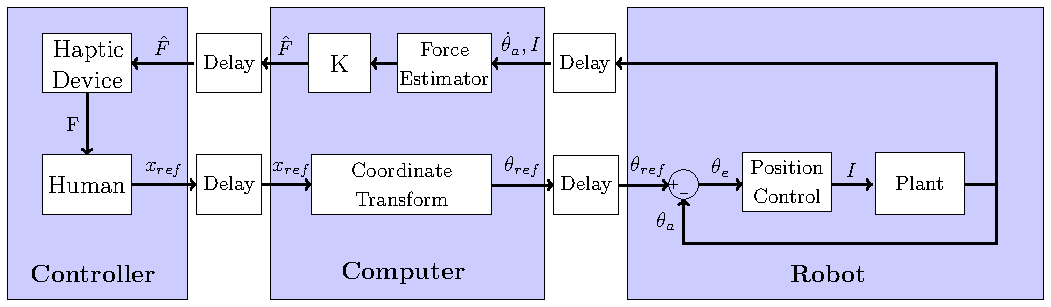
\includegraphics[width=\textwidth]{../Worksheets/rapport/pictures/control.pdf}


\begin{minipage}{0.5\linewidth}
\subsection*{Control}
\begin{itemize}
\item As shown in Fig. 2, the computer sends references to both the controller and the robot. The local controllers handle it.
\item To control the position of the tool, cascade control of position, velocity and current is used.
\end{itemize}
\end{minipage}

\begin{minipage}{0.5\linewidth}
\subsection*{Force estimation}
\begin{itemize}
	\item The force has to be estimated through the measurement of the current, velocity and position. As the tool is highly nonlinear, a linear model is not sufficient to have a good estimation of the force.
	\item The model is built using the Hammerstein-Wiener method. The linear model required for this method is built through black-box identification using the subspace method.
\end{itemize}
\end{minipage}
